% This is a LaTeX thesis template for Adam Mickiewicz University.
% to be used with Rmarkdown
% This template was produced by Jakub Nowosad
% Version: 16 February 2020

% Inspired by:
% This is a LaTeX thesis template for Monash University.
% to be used with Rmarkdown
% This template was produced by Rob Hyndman
% Version: 6 September 2016

\documentclass{amuthesis}
% \usepackage[polish]{babel}
\usepackage{polski}
\renewcommand{\figurename}{Rycina} % Redefine default figure caption %
\renewcommand{\tablename}{Tabela} % Redefine default table caption %
%%%%%%%%%%%%%%%%%%%%%%%%%%%%%%%%%%%%%%%%%%%%%%%%%%%%%%%%%%%%%%%
% Add any LaTeX packages and other preamble here if required
%%%%%%%%%%%%%%%%%%%%%%%%%%%%%%%%%%%%%%%%%%%%%%%%%%%%%%%%%%%%%%%
\usepackage{booktabs,tabularx} % Allows kableExtra to work %
\usepackage{indentfirst} % Adds indent in the first paragraph %
\usepackage{bookmark} % Adds indent in the first paragraph %

\author{Błażej Kościański}
\title{Porównanie metod (miar?) określania zmian struktury przestrzennej
kategorii pokrycia terenu}
\def\titleeng{TODO}
\def\degreetitle{Praca magisterska}
\def\major{Geoinformacja}
\def\albumid{444861}
\def\thesisyear{2023}

% Add subject and keywords below
\hypersetup{
     %pdfsubject={The Subject},
     %pdfkeywords={Some Keywords},
     pdfauthor={Błażej Kościański},
     pdftitle={Porównanie metod (miar?) określania zmian struktury
przestrzennej kategorii pokrycia terenu},
     pdfproducer={quarto with LaTeX}
}

\bibliography{thesis.bibpackages.bib}

\begin{document}

\pagenumbering{arabic}

\titlepage

\bookmarksetup{startatroot}

\hypertarget{streszczenie}{%
\chapter*{Streszczenie}\label{streszczenie}}
\addcontentsline{toc}{chapter}{Streszczenie}

\markboth{Streszczenie}{Streszczenie}

\textbf{Abstrakt}

Streszczenie powinno przedstawiać skrótowo główny problem pracy i jego
rozwiązanie. Możliwa struktura streszczenia to: (1) 1-3 zdania wstępu do
problemu (czym się zajmujemy, dlaczego jest to ważne, jakie są
problemy/luki do wypełnienia), (2) 1 zdanie opisujące cel pracy, (3) 1-3
zdania przedstawiające użyte materiały (dane) i metody (techniki,
narzędzia), (4) 1-3 zdania obrazujące główne wyniki pracy, (5) 1-2
zdania podsumowujące; możliwe jest też określenie dalszych
kroków/planów.

Słowa kluczowe: (4-6 słów/zwrotów opisujących treść pracy, które nie
wystąpiły w tytule)

\textbf{Abstract}

The abstract must be consistent with the above text.

Keywords: (as stated before)

\newpage

\setstretch{1.2}\sf\tighttoc\doublespacing

\bookmarksetup{startatroot}

\hypertarget{sec-wprowadzenie}{%
\chapter{Wprowadzenie}\label{sec-wprowadzenie}}

Informacje geograficzne stanowią wyniki selekcji i przetwarzania danych
\textbf{dotyczących aspektów} otaczającej nas przestrzeni geograficznej.
Pozwalają na bardziej zrozumiałe i efektywne analizowanie, modelowanie
oraz interpretowanie złożonych zjawisk i procesów zachodzących w naszym
otoczeniu. Informacje geograficzne i ich aspekty nie stanowią
niepodważalnych faktów, lecz często powstają w wyniku działań jednostek,
jak i wspólnych wysiłków grup ekspertów, którzy zajmują się wyborem,
analizą i klasyfikacją danych geograficznych \autocite{WhatIsLandCover}.
W procesie tworzenia informacji geograficznych istnieje zatem pewien
stopień subiektywności, który może wpłynąć na ostateczny kształt
(ostateczną postać?) tych informacji, ich interpretację, jak i na ich
użyteczność w kontekście innych zastosowań. Przykładem informacji
geograficznej, której ostateczna postać zależna jest od założeń
przyjętych w trakcie tworzenia danych przestrzennych, jest pokrycie
terenu.

Przyjmuje się, że termin pokrycie terenu obejmuje zbiór wszelkich
elementów obecnych na powierzchni Ziemi (\textbf{dodać ref}). W elementy
pokrycia terenu włączają się obiekty związane z działalnością człowieka,
skutkami sił przyrody oraz wszelkie inne istniejące obiekty, które mogą
znaleźć się w przestrzeni geograficznej (\textbf{dodać ref}). Tworzenie
dokładnych i wiarygodnych danych dotyczących pokrycia terenu jest
niezbędne w kontekście wielu zastosowań, takich jak planowanie
przestrzenne (\textbf{dodać ref}), ochrona środowiska (\textbf{dodać
ref}), czy analiza zmian klimatycznych (\textbf{dodać ref}). Ostateczna
forma tych danych jest jednak w dużej mierze determinowana przez wybory
i założenia dokonywane w procesie ich tworzenia (\textbf{ewentualnie
dodać rycinę z przykładem mapy pokrycia terenu}). W tym kontekście,
analiza pokrycia terenu staje się istotnym polem badań, które skupia się
na zarówno na technicznych aspektach zbierania danych, jak i na ich
semantycznej interpretacji (\textbf{dodać ref}).

\textbf{w tym akapicie gdzieś wspomnieć o rastrach} Dane oraz wynikowe
mapy pokrycia terenu są rezultatem złożonego procesu przetwarzania i
analizy danych przestrzennych najczęściej w postaci obrazów
satelitarnych (\textbf{dodać ref}). Na początku tego procesu, satelity
wyposażone w sensory rejestrują obrazy Ziemi z różnych zakresów
widmowych. Uzyskane obrazy mogą być interpretowane manualnie przez grupy
specjalistów. Pozwala to na uzyskanie map pokrycia terenu o wysokiej
dokładności, kosztem długiego procesu ich tworzenia (\textbf{dodać
ref}). Dużo mniej czasochłonną metodą jest przetwarzanie przy użyciu
algorytmów. Umożliwiają one względnie szybką, półautomatyczną
identyfikację i klasyfikację różnych typów powierzchni kosztem mniejszej
dokładności mapy wynikowej (\textbf{dodać ref}). Ostatecznie, dane
przekształcone w mapy pokrycia terenu mogą posłużyć do analiz zmian
pokrycia terenu (\textbf{dodać ref}).

Celem analiz zmian pokrycia terenu jest przede wszystkim monitorowanie i
pogłębienie aktualnej wiedzy na temat ewolucji otaczającego nas
krajobrazu (\textbf{dodać ref}). Jest to istotne w kontekście ochrony
przyrody (\textbf{dodać ref}), planowania przestrzennego (\textbf{dodać
ref}), oceny wpływu inwestycji (\textbf{dodać ref}) i infrastruktury na
środowisko (\textbf{dodać ref}), a także w badaniach naukowych
dotyczących zmian klimatycznych (\textbf{dodać ref}), bioróżnorodności
(\textbf{dodać ref}) oraz innych procesów ekologicznych
\autocite{ChangeDetectionTechniques}. Dzięki analizie zmian pokrycia
terenu można identyfikować obszary zagrożone degradacją, monitorować
skutki urbanizacji, deforestacji czy erozji, co umożliwia podejmowanie
odpowiednich działań w celu zrównoważonego zarządzania środowiskiem i
zachowaniem jego integralności.

W badaniach nad zmianami pokrycia terenu wykorzystuje się różnorodne
metody analityczne \autocite{ChangeDetectionTechniques}. Niemniej
jednak, wiele z tych technik koncentruje się na analizie zmian na
poziomie indywidualnych komórek w siatce rastra (\textbf{dodać ref}).
Choć podejście to może dostarczać użytecznych informacji dotyczących
trendów zmian pokrycia terenu na niewielkich obszarach, charakteryzuje
się ono istotnymi ograniczeniami w kontekście interpretacji wyników.
Szczególnie w przypadku badań obejmujących rozległe terytoria, takie jak
kraje czy nawet kontynenty, bardziej efektywne staje się zastosowanie
metod opartych na analizie struktur przestrzennych
\autocite{Netzel2015}. Głównym założeniem tych metod jest
przekształcenie danych z postaci pojedynczych wartości komórek rastra w
sygnatury przestrzenne, a następnie \textbf{DOPISAĆ}

Sygnatury przestrzenne stanowią statystyczny opis struktur
przestrzennych kategorii pokrycia terenu na mniejszych, wydzielonych
obszarach w obrębie całego zbioru danych. W celu porównania ze sobą
dwóch sygnatur przestrzennych, wykorzystywane są miary niepodobieństwa.
Umożliwiają one określenie w jakim stopniu dwa analizowane obszary się
od siebie różnią pod względem \textbf{DOPISAĆ} Opracowane zostało wiele
różnych miar niepodobieństwa, takich jak odległość euklidesowa,
odległość Canberra, metryka Wave Hedges, współczynnik podobieństwa
Jaccarda, odległość Jensena-Shannona czy dywergencja Pearsona
\autocite{Cha2007}. Współcześnie jednak nie określono, która z tych miar
jest najbardziej zgodna zarówno z postrzeganiem przez człowieka, jak i
wpływem zmian na procesy środowiskowe.

Celem tej pracy było porównanie metod określania zmian struktury
przestrzennej kategorii pokrycia terenu w kontekście ich korelacji z
postrzeganiem zmian przestrzennych przez ludzi. W celu realizacji tego
zadania przeprowadzone zostały ankiety, w których zadaniem respondentów
było określenie stopnia podobieństwa między parami rastrów. Badania
przeprowadzone zostały na rastrach składających się wyłącznie z dwóch
lub trzech kategorii. Wyniki ankiety zestawione zostały z wartościami 46
miar niepodobieństwa. Na tej podstawie, do dalszej analizy wybrane
zostało 8 miar niepodobieństwa charakteryzujących się największą
zgodnością z ludzką percepcją zmian przestrzennych.

\bookmarksetup{startatroot}

\hypertarget{sec-lit}{%
\chapter{Metody określania zmian struktur
przestrzennych}\label{sec-lit}}

W tym rozdziale zostaną kolejno opisane wszystkie zagadnienia kluczowe
do pełnego zrozumienia tematyki określania zmian struktur przestrzennych
w kontekście tematu zmian pokrycia terenu. W pierwszej kolejności
zostanie opisana tematyka wykorzystania teorii informacji w analizie
zmian pokrycia terenu. Omówione zostaną koncepcje przestrzennej
kompozycji oraz konfiguracji, a także miary umożliwiające ich
obliczenie. Następnie opisana zostanie idea reprezentacji rastrów w
postaci macierzy i wektorów współwystępowania. W końcowej części
rozdziału wyjaśnione zostaną zagadnienia miar odległości i podobieństwa
oraz ich wykorzystania w celach analiz przestrzennych.

\hypertarget{analiza-zmian-struktur-przestrzennych}{%
\section{Analiza zmian struktur
przestrzennych}\label{analiza-zmian-struktur-przestrzennych}}

Zmiany i różnice w pokryciu terenu można analizować przy użyciu różnych
metod. Najbardziej podstawowym sposobem jest prosta analiza ilościowa
różnic w pokryciu terenu na analizowanym obszarze lub obszarach. Inny
sposób, oparty o metody wywodzące się z dziedziny ekologii krajobrazów,
polega na sprowadzeniu rastrów do postaci sygnatur przestrzennych.
Sygnatury te stanowią statystyczny opis pewnych struktur przestrzennych
występujących wewnątrz rastra \autocite{nowosad_motif,Jasiewicz_GeoPAT}.
Takie podejście do analizy przestrzennej umożliwia między innymi ocenę
różnic w przestrzennej kompozycji i konfiguracji analizowanych jednostek
przestrzennych.

Najbardziej fundamentalną sygnaturą przestrzenną rastra jest kompozycja.
Opisuje ona liczbę komórek każdej kategorii wewnątrz analizowanego
rastra. Kolejną ważną sygnaturą przestrzenną jest konfiguracja, która w
sposób liczbowy opisuje sąsiadowanie ze sobą poszczególnych kategorii
rastra \autocite{Gustafson1998}. Często w celu lepszej reprezentacji
analizowanych rastrów możemy wykorzystywać także bardziej skomplikowane
sygnatury. Przykładem sygnatury łączącej zarówno kompozycję, jak i
konfigurację przestrzenną jest macierz współwystępowania. Jest to
macierz o wymiarach k na k, gdzie k reprezentuje liczbę kategorii
obecnych w analizowanym rastrze
\autocite{Haralick_1973,Jasiewicz_GeoPAT}. Macierz tą możemy
skonstruować poprzez zliczanie kolejno wszystkich par sąsiadujących ze
sobą komórek w rastrze. Wewnątrz tej macierzy, wartości ułożone na
przekątnych odnoszą się do kompozycji rastra, natomiast pozostałe do
jego konfiguracji.

Na podstawie macierzy współwystępowania mogą zostać obliczone różne
miary wywodzące się z dziedziny teorii informacji. Przykładem takiej
miary jest entropia, która opisuje zróżnicowanie kompozycji rastra,
czyli udziałów każdej z kategorii w rastrze. Kolejną miarą jest względna
informacja wzajemna. Reprezentuje ona stopień sąsiadowania ze sobą
kategorii w rastrze, czyli jego konfigurację przestrzenną. W celu
porównywania ze sobą sygnatur w postaci dwuwymiarowej macierzy należy je
sprowadzić do postaci jednowymiarowego wektora, a następnie
przeprowadzić jego normalizację, tak aby wszystkie wartości sumowały się
do 1. Taka postać pozwala na obliczanie miar odległości lub
podobieństwa, pozwalających na porównywanie histogramów wartości
\autocite{Cha2007}. Miary te następnie pozwalają określić stopień
zróżnicowania dwóch rastrów. Podejście to może być także wykorzystane w
innych analizach przestrzennych, jak wyszukiwanie obszarów o podobnej
strukturze przestrzennej, wykrywanie ich zmian oraz grupowanie obszarów
o podobnej strukturze przestrzennej \autocite{nowosad_motif}.

\hypertarget{miary-odlegux142oux15bci-podobieux144stwa-i-niepodobieux144stwa}{%
\section{Miary odległości, podobieństwa i
niepodobieństwa}\label{miary-odlegux142oux15bci-podobieux144stwa-i-niepodobieux144stwa}}

Odległość i rozbieżność (inaczej podobieństwo) stanowią pewien
policzalny stopień zróżnicowania pary obiektów. Największą różnicą
między nimi jest to, że odległości są symetryczne, podczas gdy
rozbieżności są niesymetryczne. Oznacza to, że wyłącznie dla miar
odległości otrzymujemy identyczny wynik przy porównywaniu par obiektów A
i B, jak i par B i A. Wybór odpowiedniej miary odległości lub
podobieństwa zależy między innymi od rodzaju pomiaru lub sposobu
reprezentacji obiektów \autocite{Cha2007}. W związku z tym rodzi się
pytanie, która z miar pozwala na uzyskanie najlepszych wyników dla
danego zastosowania. Celem tej pracy, jak wspomniano we Wprowadzeniu,
jest zatem wskazanie takich miar odległości lub podobieństwa, których
zmiany wartości są najbardziej powiązane z postrzeganiem tych samych
zmian przez człowieka.

Zagłębiając się w tematykę miar odległości i podobieństwa należy przede
wszystkim wyjaśnić nieścisłości wynikających z samego ich nazewnictwa.
Wykorzystanie w tej pracy samej nazwy ``miary odległości'' mogłoby być
zinterpretowane jako grupa miar pozwalających na określenie
rzeczywistego, mierzalnego dystansu pomiędzy dwoma obiektami, co nie
jest zgodne z tym w jaki sposób miary te wykorzystane zostały w tej
pracy. Nazwa ``miary podobieństwa'' jest natomiast sprzeczna w
interpretacji z ludzką intuicją. Logiczne byłoby, że niskie wartości tej
miary oznaczają małe podobieństwo, podczas gdy wysokie wartości
oznaczają wysokie podobieństwo między porównywanymi obszarami. W
rzeczywistości miary podobieństwa funkcjonują zupełnie przeciwnie. W
związku z powyższymi problemami, wszystkie 45 miar odległości,
podobieństwa oraz tych wywodzących się z dziedziny teorii informacji,
które zostały wykorzystane w tej pracy będą dalej nazywane miarami
niepodobieństwa. Nazwa ta, o ile pozornie trudniejsza do zrozumienia ma
jednak istotną przewagę w kontekście wszelkich analiz. W tym kontekście,
wraz ze wzrostem wartości miar niepodobieństwa rośnie różnica pomiędzy
porównywanymi obszarami. Oznacza to, że niskie wartości miar
niepodobieństwa wskazują na niskie niepodobieństwo, czyli niewielkie
różnice między porównywanymi obszarami. Analogicznie, wysokie wartości
miar niepodobieństwa wskazują na duże różnice między porównywanymi
obszarami.

Na podstawie podobieństw syntaktycznych, wyróżnia się kilka grup rodzin
miar niepodobieństwa: rodzina Minkowski (odległość euklidesowa,
odległość Minkowskiego, odległość Manhattan), rodzina L1 (Canberra,
Sorensen, Kulczynski), rodzina Intersection (Intersection, Wave Hedges,
Ruzicka), rodzina Inner Product (Jaccard, Harmonic mean), rodzina
Squared-chord (Fidelity, Matusita), rodzina Squared L2 (Clark, Pearson
X2, Neyman X2), rodzina Shannon's Entropy (Jensen-Shannon,
Kullback-Leibler), a także miary będące połączeniem innych miar oraz
miary wywodzące się z teorii informacji.

\textbf{\emph{tu mi się skończyły pomysły}}

\bookmarksetup{startatroot}

\hypertarget{sec-materialy}{%
\chapter{???}\label{sec-materialy}}

\bookmarksetup{startatroot}

\hypertarget{sec-wyniki1}{%
\chapter{Pierwsza ankieta}\label{sec-wyniki1}}

W tym rozdziale zostanie omówiony cel przeprowadzenia pierwszej ankiety
oraz istotne aspekty związane z jej formą. Następnie opisany zostanie
sposób przygotowania danych wraz z przyjętą metodą doboru pytań do
ankiety. W końcowej części rozdziału przeprowadzona zostanie analiza i
podsumowanie wyników uzyskanych z ankiety. Wyniki zostaną zestawione z
miarami niepodobieństwa uwzględnionymi w analizie oraz zostaną
przedstawione pierwsze wnioski wynikające z przeprowadzonych analiz.

Pierwsza ankieta została przeprowadzona w celu uzyskania wstępnych
informacji, mających na celu zrozumienie wpływu różnic w entropii oraz
względnej informacji wzajemnej między parami analizowanych rastrów na
postrzeganie zmian pokrycia terenu przez ludzi. Głównym celem badania
było wykazanie potencjalnych związków między percepcją zmian w pokryciu
terenu przez ludzi a miarami niepodobieństwa, które te zmiany
kwantyfikują. Przeprowadzenie ankiety pozwoliło także na wyznaczenie
dalszego kierunku badań, jak i celów, które miałyby zostać osiągnięte
jako wynik kolejnej ankiety.

Badanie zostało realizowane w terminie od 21 do 24 listopada 2022 roku.
Proces zbierania odpowiedzi respondentów przyjął formę ankiety online,
co pozwoliło respondentom na wygodny udział w badaniu przy użyciu
komputera lub urządzenia mobilnego. Ankieta stworzona została w formie
aplikacji internetowej za pomocą języka programowania R, na podstawie
pakietów shiny oraz shinysurveys. Sama aplikacja umieszczona została na
platformie shinyapps.io (https://www.shinyapps.io/). Przeprowadzenie
ankiety w formie online umożliwiło systematyczne gromadzenie oraz
przechowywanie odpowiedzi w formie tabelarycznej, ułatwiając tym samym
dalszą analizę i interpretację danych. Respondenci stanowili grupę 50
studentów Wydziału Nauk Geograficznych i Geologicznych Uniwersytetu im.
Adama Mickiewicza. Wybór tej grupy respondentów oznacza, że byli oni już
zaznajomieni z tematyką tworzenia i analiz map w formie rastrowej oraz
pojęciem zmian pokrycia terenu.

Każdy z ankietowanych otrzymał do wypełnienia jeden z dwóch wcześniej
przygotowanych zbiorów pytań. Każdy ze zbiorów składał się z 48 pytań,
przy czym część pytań między zbiorami się pokrywała. Oznacza to, że
łącznie uzyskano odpowiedzi na 93 unikatowe pytania. W każdym z pytań
zadaniem respondentów było określenie podobieństwa na podstawie dwóch
załączonych rastrów. W ramach badania respondenci mieli możliwość
wyrażania swoich odpowiedzi za pomocą pięciostopniowej skali Likerta,
która obejmowała poziomy od ``Brak'' przez ``Bardzo małe'',
``Umiarkowane'', ``Bardzo duże'' aż po ``Pełne''. Wykorzystanie skali
Likerta o nieparzystej liczbie przedziałów, pozwoliło na zastosowanie
przedziału środkowego, którego celem było reprezentowanie odpowiedzi
neutralnych lub trudnych do określenia. Początkowo, zamiast skali
Likerta planowano wykorzystać skalę liczbową, w zakresie mieszczącym się
od 1 do 100, jednakże zrezygnowano z tego pomysłu, jako że znaczenie
wartości na skali liczbowej może być interpretowane inaczej przez
każdego respondenta oraz skala ta nie pozwala na uwzględnienie
wspomnianej wcześniej odpowiedzi neutralnej. Przykład pytania
przedstawionego respondentom ilustruje rycina
\ref{fig-przyklad_pytania}.

\begin{figure}[t]

{\centering 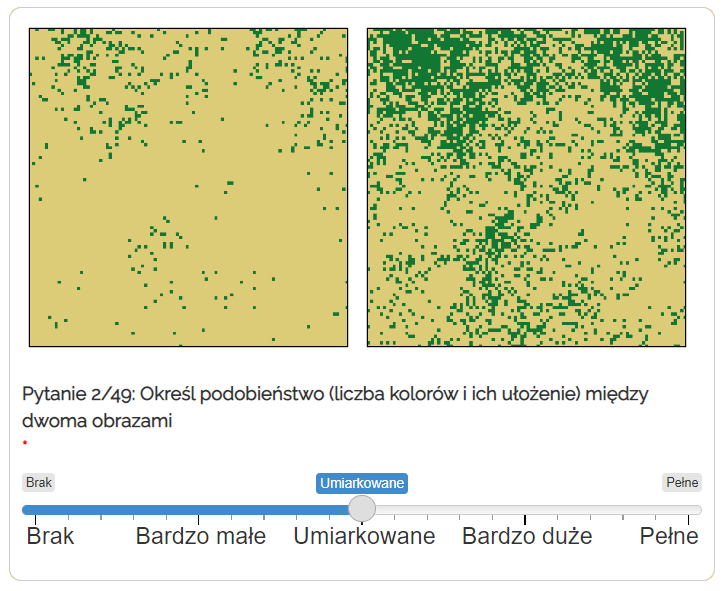
\includegraphics[width=1\textwidth,height=4.6875in]{figures/przyklad_pytania.png}

}

\caption{\label{fig-przyklad_pytania}Przykładowe pytanie z pierwszej
ankiety}

\end{figure}

\hypertarget{dane-i-format-pytaux144}{%
\section{Dane i format pytań}\label{dane-i-format-pytaux144}}

Najważniejszym założeniem przy tworzeniu zbioru rastrów do pierwszej
ankiety było przygotowanie ich w sposób umożliwiający uzyskanie pełnej
reprezentacji wszystkich możliwych wartości przestrzennej kompozycji,
jak i konfiguracji. Zbiór rastrów został przygotowany w oparciu o
wykorzystanie funkcji \emph{nlm\_fbm} z pakietu NLMR
\autocite{NLMR2018}. Funkcja ta pozwala na symulację rastrów przy użyciu
ułamkowych ruchów Browna, będących uproszczeniem ruchów Browna. W tej
funkcji poziom korelacji między kolejnymi krokami jest kontrolowany za
pomocą parametru ``frac\_dim''. W kontekście tego badania, parametr ten
reguluje konfigurację przestrzenną. Oznacza to, że w przypadku, gdy
``frac\_dim'' przyjmuje niską wartość, wartości w generowanym rastrze
rozmieszczone są w sposób losowy, zbliżony do szumu. Natomiast w
przypadku wysokiej wartości ``frac\_dim'', na wynikowym rastrze tworzą
się skupiska najwyższych i najniższych wartości, a przejścia pomiędzy
nimi mają płynny, wygładzony charakter. \textbf{\emph{tutaj dodać
kawałek kodu pokazujący jak działa funkcja?}} Kolejnym krokiem w
procesie tworzenia danych było dodanie zróżnicowania rastrów na
podstawie ich przestrzennej kompozycji. Zostało to osiągnięte poprzez
podział każdego z wynikowych rastrów na kategorie w oparciu o stałe
przedziały wartości dla wszystkich rastrów. Proces

\begin{figure}[t]

{\centering 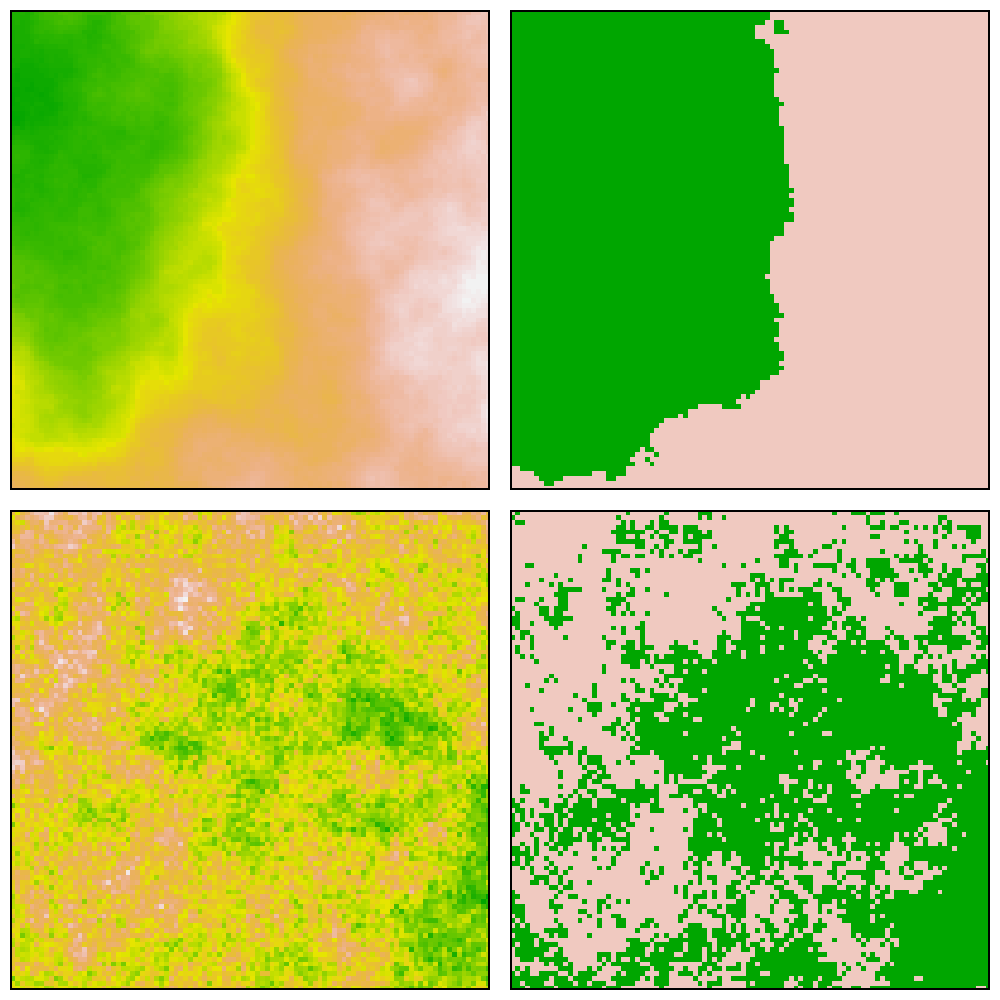
\includegraphics[width=4.16667in,height=4.16667in]{figures/wykres2_gen.png}

}

\caption{\label{fig-wykres2_gen}Wizualizacja procesu symulacji rastrów
do pierwszej ankiety albo placeholder zamiast pokazania jak działa
funkcja}

\end{figure}

W następnym etapie przygotowania danych obliczone zostały wybrane miary
opisujące struktury przestrzenne: entropia (ent), informacja wzajemna
(mutinf) oraz względna informacja wzajemna (relmutinf). Miary te
umożliwiły potwierdzenie uzyskania oczekiwanego rozkładu kompozycji i
konfiguracji wewnątrz zbioru rastrów. Ostatecznie wygenerowane zostały
zbiory rastrów składających się wyłącznie z dwóch lub trzech kategorii
pokrycia terenu. Przykład jednego ze zbiorów rastrów przedstawia rycina
\ref{fig-wykres1_2classes}. Celem uwzględnienia w badaniu rastrów z
większą liczbą kategorii było stwierdzenie potencjalnych zależności
między liczbą kategorii na rastrach a postrzeganiem przez ankietowanych
podobieństw w strukturach przestrzennych.

Ostatnim krokiem przygotowania danych było wybranie najbardziej
reprezentatywnych par rastrów tworzących poszczególne pytania. W tym
celu, pytania w ankietach podzielone zostały na na dwie grupy, wewnątrz
których znalazły się po trzy podgrupy pytań. W pierwszej kolejności
respondenci zetknęli się z 24 pytaniami dotyczącymi rastrów
uwzględniających wyłącznie dwie kategorie pokrycia terenu, a następnie z
24 pytaniami uwzględniającymi trzy kategorie pokrycia terenu. Pierwsza
podgrupa pytań (6 par rastrów) składała się z par rastrów różniących się
między sobą wyłącznie entropią. Podgrupa druga (6 par rastrów) zawierała
wyłącznie rastry różniące się względną informacją wzajemną. Ostatnia
podgrupa (12 par rastrów) składała się z pytań zróżnicowanych zarówno
pod względem entropii, jak i względnej informacji wzajemnej. Taki sposób
doboru pytań pozwolił na zredukowanie liczby odpowiedzi wymaganych od
respondentów, jak i ograniczenie wpływu błędu selekcji, który powstałby
w wyniku niewłaściwego doboru pytań. Respondenci celowo nie zostali
poinformowani o występujących różnicach pomiędzy kolejnymi pytaniami,
ponieważ mogłoby mieć to wpływ na udzielane przez nich odpowiedzi, co z
kolei mogłoby wpłynąć na ostateczne wyniki badania.

\begin{figure}[t]

{\centering 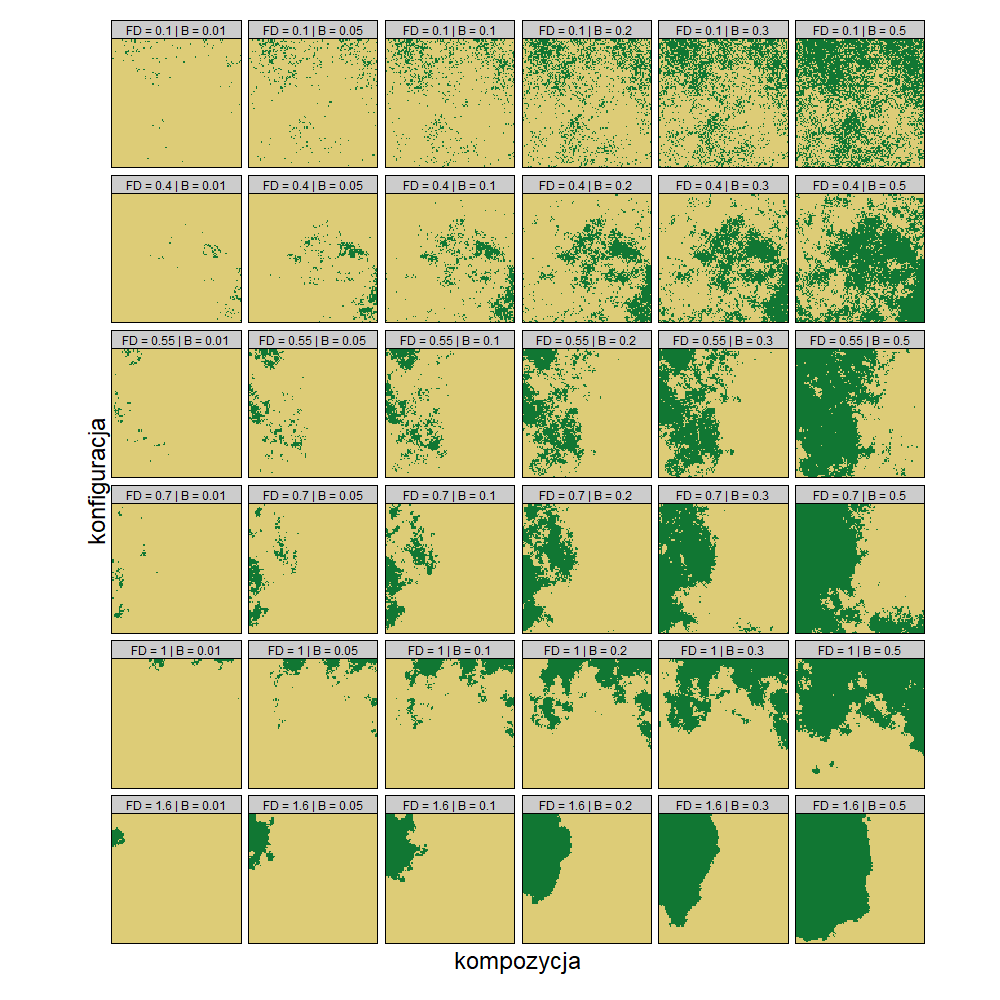
\includegraphics[width=1\textwidth,height=5.20833in]{figures/wykres1_2classes.png}

}

\caption{\label{fig-wykres1_2classes}Przykład zbioru wygenerowanych
rastrów (2 kategorie pokrycia terenu)}

\end{figure}

\hypertarget{wyniki}{%
\section{Wyniki}\label{wyniki}}

Łącznie uzyskane zostało 2400 odpowiedzi na pytania z ankiety.
Podsumowanie uzyskanych odpowiedzi przedstawione zostało w tabeli 1.
Według ankietowanych prawie 36\% par rastrów charakteryzowała się
brakiem podobieństwa, 32.6\% uzyskanych odpowiedzi wskazywało na bardzo
małe podobieństwo, 18.1\% na umiarkowane, 11.6\% bardzo duże, natomiast
mniej niż 2\% wskazywało na pełne podobieństwo. Warto tutaj także
zwrócić uwagę, że zestawienia wszystkich odpowiedzi w zależności od
liczby kategorii widocznych na rastrach nie wskazują na znaczące różnice
w liczbie odpowiedzi dla danej kategorii. Największą różnicę stanowi w
tym przypadku kategoria ``Bardzo duże'', dla której liczba odpowiedzi
dla rastrów z dwoma i trzema kategoriami pokrycia terenu różni się
zaledwie o 2.7\%. Najmniejszą różnicą charakteryzuje się kategoria
``Pełne'', gdzie liczba odpowiedzi pomiędzy zestawami różni się o jedyne
0.9\%.

Poziom zgodności każdego pytania został obliczony jako stosunek
najczęściej udzielonej odpowiedzi względem całkowitej liczby odpowiedzi.
Całkowity poziom zgodności ankietowanych został oszacowany na 55\%.
Oznacza to, że 1321 z 2400 udzielonych odpowiedzi znajdowało się w
grupie najczęstszej odpowiedzi dla danego pytania. Pytania różniące się
zarówno entropią, jak i względną informacją wzajemną cechowały się
najwyższym poziomem zgodności odpowiedzi wynoszącym 61\%, podczas gdy
pytania różniące się wyłącznie entropią uzyskały wynik 53\%, a pytania
różniące się wyłącznie względną informacją wzajemną uzyskały wynik 52\%.
Najwyższy poziom zgodności odpowiedzi osób ankietowanych wyniósł 92\% i
dotyczył pytania różniącego się zarówno entropią, jak i względną
informacją wzajemną (dopisać jak bardzo różniły się ent i rmi).
Najniższy poziom zgodności, czyli zaledwie 38\%, osiągnęło aż 8 pytań.
Wyłącznie dwa z nich dotyczyły pytań zawierających trzy kategorie
pokrycia terenu, podczas gdy pozostałe - dwóch. 75\% z tych pytań
uwzględniało rastry różniące się pod względem względnej informacji
przestrzennej (inna konfiguracja) przy zachowaniu tej samej entropii
(identyczna kompozycja).

W końcowym etapie analizy wyniki uzyskane z przeprowadzonej ankiety
zostały zestawione z wynikami 45 różnych miar niepodobieństwa dla par
rastrów uwzględnionych w ankiecie. Aby ocenić relacje między
najczęstszymi odpowiedziami uczestników ankiety a miarami
niepodobieństwa, przeprowadzono analizę korelacji Pearsona. W ten sposób
uzyskano ostateczny ranking miar, który został przedstawiony w Tabeli 1.
Na podstawie analizy korelacji można wywnioskować, że spośród 45
uwzględnionych w badaniu metod obliczania podobieństwa między parami
rastrów, jedynie 6 z nich wykazuje dodatnią korelację z wynikami
uzyskanymi z ankiety. Spośród wszystkich metod, najwyższą wartość
korelacji osiągnęła metoda Fidelity ze współczynnikiem korelacji równym
0,34. Ponadto, miary ``harmonic mean'' i ``intersection'' również
wykazały dość wysoki współczynnik korelacji. Jak wspomniano wyżej, nie
wszystkie miary odległości charakteryzowały się dodatnim współczynnikiem
korelacji. Miary ``canberra'', ``divergence'' i ``clark'' wykazały
współczynniki korelacji poniżej -0,4, co wskazuje na ich umiarkowaną,
ujemną zależność z wynikami ankiety. Oznacza to, że miary te wskazują na
wysokie podobieństwo par rastrów, które ludzie określiliby jako zupełnie
niepodobne i vice versa. Pytania dotyczące rastrów uwzględniających
wyłącznie dwie kategorie pokrycia terenu z reguły charakteryzują się
wyższym współczynnikiem korelacji z najczęstszymi odpowiedziami
ankietowanych niż pytania z podziałem na trzy kategorie pokrycia terenu.
Może to być wynikiem tego, że ludziom może łatwiej przychodzić
określenie różnicy w rastrach, które zawierają mniejszą ilość
informacji. Jedyny wyjątek stanowią w tej sytuacji wyłącznie miary,
które osiągnęły najniższe wartości współczynnika korelacji. Dla rastrów
z trzema kategoriami osiągnęły one jeszcze niższy współczynnik na
poziomie nawet -0,77. Ich wyniki wskazują na silne, ujemne związki
między analizowanymi zmiennymi.

Otrzymane wartości współczynników korelacji nie pozwalają na definitywne
stwierdzenie na istnienie liniowych relacji pomiędzy metodami określania
niepodobieństwa a opinią człowieka, przynajmniej na podstawie analizy
symulowanych danych rastrowych. Dotychczasowe wyniki dają ogólny zarys
relacji miar niepodobieństwa do ludzkiej percepcji, w związku z czym w
kolejnym etapie sporządzona została ankieta w pełni opierająca się o
rzeczywiste dane rastrowe.

Przeanalizowane wyniki pierwszej ankiety wraz z opisem przyjętej
metodyki projektu przedstawione zostały na posterze konferencyjnym
pt.~„Porównanie metod określania zmian struktury przestrzennej kategorii
pokrycia terenu'', autorstwa Błażeja Kościańskiego oraz dra hab. Jakuba
Nowosada. Poster został przedstawiony w trakcie sesji posterowej na
konferencji Geoinformacja: Nauka - Praktyka - Edukacja
(https://geoinformacja20uam.pl/), odbywającej się w dniach 1-3 grudnia
2022 roku na Wydziale Nauk Geograficznych i Geologicznych im. Adama
Mickiewicza w Poznaniu.

\bookmarksetup{startatroot}

\hypertarget{sec-wyniki2}{%
\chapter{Druga ankieta}\label{sec-wyniki2}}

\bookmarksetup{startatroot}

\hypertarget{podsumowanie}{%
\chapter{Podsumowanie}\label{podsumowanie}}

\printbibliography[heading=bibintoc, title=Bibliografia]

\end{document}
